\externaldocument{algoritmoscomparados}

\chapter[Análise dos Resultados]{Análise dos Resultados}
\label{resultados}
% ----------------------------------------------------------
Neste capítulo, iremos analisar o desempenho dos algoritmos descritos no capítulo anterior. A comparação e determinação de qual algoritmo possui o melhor desempenho será feita utilizando a métrica de satisfação do usuário (a qual foi definida na seção \ref{Satisfacao}). Inicialmente, iremos apresentar os parâmetros utilizados na simulação e posteriormente mostraremos os resultados e discussão destes resultados.

\section{Parâmetros da simulação}

\subsection{Parâmetros gerais}

O ambiente de simulação utilizado neste trabalho leva em consideração as principais características dos sistemas celulares 4G baseados em OFDMA. No capítulo \ref{Simulacao}, descrevemos as características do nosso simulador. Na tabela \ref{Tab:Gen_Simul_Param} são mostrados os parâmetros gerais de simulação utilizados.

\renewcommand{\arraystretch}{1}
\begin{table}[!ht]
	\centering
	\begin{threeparttable}[t]
		\caption{Parâmetros gerais da simulação.}
		\label{Tab:Gen_Simul_Param}
		\centering
		\tiny
		\begin{tabular}{l l}
			\toprule
			\textbf{Parâmetro} & \textbf{Valor}\\
			\midrule
			Potência máxima de transmissão da BS\tnote{a} & 12 W \cite{3gpp.36.814}\\
			\midrule
			Setorização da antena da BS & 3 setores de 120$^{\circ}$ \cite{3gpp.36.814}\\
			\midrule
			Raio da célula & 1 km\\
			\midrule
			Velocidade dos dispositivos móveis & 3 km/h \cite{3gpp.25.814}\\
			\midrule
			Largura de banda do sistema & 3 MHz \cite{Book:Pelcat2013}\\
			\midrule
			Quantidade de RBs & 15 \cite{Book:Pelcat2013}\\
			\midrule
			Tempo de coerência do canal & 90 ms\\
			\midrule
			Ganho da antena\tnote{b} & $G_{h}(\theta_{h}) + G_{v}(\theta_{v}$) \cite{Gunnarsson2008}\\
			\midrule
			Ângulo de \textit{Downtilt} & 8$^{\circ}$\\
			\midrule
			Desvio padrão do sombreamento lognormal ($\sigma_{\mathrm{sh}}$) & 8 dB \cite{3gpp.25.814}\\
			\midrule
			Desvanecimento de pequena escala & 3GPP \textit{Typical Urban} \cite{3gpp.25.943}\\
			\midrule
			Potência AWGN por subportadora & -123.24 dBm\\
			\midrule
			Figura de ruído & 9 dB\\
			\midrule
			Limite de SNR da MCS 1 & -6.9 dB \cite{EUSIPCO2009}\\
			\midrule
			Degradação da CSI ($\psi$) & 0,05\\
			\midrule
			Atraso da CSI ($\Delta n$) & 15 TTIs\\
			\midrule
			Tempo da sessão de simulação & 30 segundos\\
			\midrule
			Número de simulação executadas & 90 \\
			\bottomrule
		\end{tabular}
		\begin{tablenotes}
			\item [a] Valor utilizado devido à quantidade de RBs utilizadas.
			\item [b] $\theta_{h}$ e $\theta_{v}$ representam os ângulos horizontal e vertical relacionados com a BS, respectivamente.
		\end{tablenotes}
		{Fonte: Elaborada pelo autor.}
	\end{threeparttable}
\end{table}

\subsection{Parâmetros dos modelos de tráfego}

A descrição dos modelos de tráfego utilizados para compor o cenário com múltiplos serviços foi apresentada no capítulo \ref{Simulacao}. No entanto, o valor dos parâmetros utilizados para os modelos de tráfego ainda não foram especificados. Na tabela \ref{Tab:Par_VOIP} mostramos os parâmetros utilizados para o tráfego VoIP e na tabela \ref{Tab:Par_CBR} mostramos os parâmetros utilizados para o tráfego CBR. 

\begin{table}[!ht]
	\centering
	\begin{threeparttable}[t]
		\caption{Parâmetros do modelo de tráfego VoIP.}
		\label{Tab:Par_VOIP}
		\centering
		\small
		\begin{tabular}[t]{ll}
			\toprule
			\textbf{Parâmetro} & \textbf{Valor}\\
			\midrule
			Tamanho do pacote & 320 bits\\
			\midrule
			Intervalo entre chegada de pacotes & 20 ms\\
			\midrule
			Duração da chamada & 30 segundos\\
			\midrule
			Média de tempo dos estados da cadeia de Markov & 1 s\\
			\midrule
			Fator de atividade & 50\%\\
			\midrule
			Limite para a FER ($\text{FER}_{\text{req}}^{\text{rt}}$)& 2\%\\
			\midrule
			Limite de tempo do pacote HOL($\Phi_{\text{req}}^{\text{rt}}$) & 20 ms\\
			\bottomrule
		\end{tabular}
		{Fonte: Elaborada pelo autor.}
	\end{threeparttable}
\end{table}

\begin{table}[!ht]
	\centering
	\begin{threeparttable}[t]
		\caption{Parâmetros do modelo de tráfego CBR.}
		\label{Tab:Par_CBR}
		\centering
		\small
		\begin{tabular}[t]{ll}
			\toprule
			\textbf{Parâmetro} & \textbf{Valor}\\
			\midrule
			Taxa de geração de pacotes & 512~kbps\\
			\midrule
			Tamanho do pacote & 2048 bits\\
			\midrule
			Intervalo entre chegada de pacotes & 4 ms\\
			\midrule
			Duração da sessão & 30 segundos\\
			\midrule
			Média de tempo dos estados da cadeia de Markov & 1 s\\
			\midrule
			Fator de atividade & 50\%\\
			\midrule
			Limite de tempo do Pacote HOL & 200 ms\\
			\midrule
			Requerimento de vazão de dados ($\Phi_{\text{req}}^{\text{nrt}}$) & 512~kbps \\
			\bottomrule
		\end{tabular}
		{Fonte: Elaborada pelo autor.}
	\end{threeparttable}	
\end{table}

\subsection{Parâmetros dos algoritmos estudados}

Como os modelos de tráfego utilizados neste trabalho são diferentes em relação aos valores dos parâmetros dos modelos analisados em \citeonline{Phd:Song2005}, \citeonline{Proc:Lei2007}, \citeonline{Nasralla2013} e \citeonline{basukala2009performance}, algumas adaptações foram feitas para que os algoritmos de comparação tivessem suas propostas mantidas. Vale ressaltar que as adaptações foram feitas considerando as propostas iniciais dos autores e as magnitudes relativas das prioridades atribuídas originalmente para cada classe de serviço fossem mantidas.    

Como o algoritmo EXP/PF não depende dos parâmetros referentes aos modelos de tráfego, este algoritmo não sofreu nenhuma modificação. Em relação ao algoritmo QHMLWDF, também não há parâmetros que dependem dos tráfegos considerado. Para o QHMLWDF, apenas foi considerado que $\alpha[n] = 0,1$, o que significa que a máxima probabilidade aceitável que os pacotes excedam o tempo limite é 10\% da quantidade total de pacotes enviados. 

Os algoritmos MDU e \textit{Utility} Lei possuem parâmetros que são definidos de acordo com os modelos de tráfego considerados. Para o algoritmo MDU, existem 3 possíveis funções de utilidade que podem ser consideradas. Como neste trabalho utilizamos o serviço VoIP e o serviço CBR, iremos utilizar as funções de utilidade referentes ao VoIP e \textit{Streaming} (uma vez que o serviço CBR pode ser considerado um tipo de \textit{streaming} com taxa constante) que foram propostas em \citeonline{Phd:Song2005}. No entanto, como os valores dos parâmetros dos modelos de tráfego são um pouco diferentes, as funções para o serviço VoIP ($ |U^{'}_V(\text{w})|$) e o serviço CBR ($|U^{'}_S(\text{w})|$) ficam:
%
\begin{equation}
\label{Eq:VoIPAlt}
\left| U^{'}_V(\text{w}) \right| = \begin{cases} 
\text{w}[n]^{2,9}, & \text{if  } \text{w}[n] \leq \text{5 ms} \\ 
\text{w}[n]^{2,9} - 5^{2,9} + 5, & \text{if  } \text{w}[n] >  \text{5 ms}; 
\end{cases}
\end{equation} 
%
\begin{equation}
\label{Eq:StreamingAtl}
\left| U^{'}_S(\text{w}) \right| = \begin{cases} 
\text{w}[n], & \text{if  } \text{w}[n] \leq \text{50 ms} \\ 
\text{w}[n]^{1,5} - 50 + 50^{1,5}, & \text{if  } \text{w}[n] >  \text{50 ms},
\end{cases}
\end{equation}
%
em que os 5~ms de $ |U^{'}_V(\text{w})|$ refere-se a 0,25\% $\cdot$ 20~ms (tempo limite do pacote HOL do VoIP) e 50~ms de $|U^{'}_S(\text{w})|$ refere-se a 0,25\% $\cdot$ 200~ms (tempo limite do pacote HOL do CBR), seguindo o que foi proposto originalmente. Dessa forma, a magnitude e prioridade relativa entre esses serviços mostradas na figura \ref{fig:WeightSong} são mantidas.
Para o algoritmo \textit{Utility} Lei, os parâmetros das funções de utilidade foram redefinidos para os seguintes valores: $\beta = 450$, $\Phi_{\text{req}}^{\text{rt}} = 20 \text{ ms}$, $a = 5$, $b = 0,5$ e $c = 200 \text{ ms}$. Com isso a magnitude e prioridade relativa entre os serviços considerados mostradas nas figuras \ref{fig:PrimitiveWeightLEI} e \ref{fig:WeightLEI} são mantidas.

\section{Resultados e discussão}

Nesta seção iremos mostrar os resultados obtidos para o desempenho dos algoritmos estudados. Como já mencionado, a métrica utilizada para realizar a comparação será a métrica de satisfação do usuário. Primeiramente iremos mostrar os resultados para cenários com serviço único e posteriormente iremos mostrar os resultados para cenários com múltiplos serviços. Todos os resultados das simulações neste trabalho são apresentados com 95\% de intervalo de confiança da média das amostras, os quais serão ilustrados como barras verticais ou horizontais em torno de um determinado ponto.  

A definição de qual algoritmo possui melhor desempenho será feita analisando o Plano de Capacidade Conjunta do sistema, que é uma ferramenta poderosa para análise de resultados, já que ela fornece uma forma completa de avaliação condensando os resultados para cenários com serviço único e múltiplos serviços em um único gráfico.

As figuras apresentadas nesta seção ilustrarão gráficos onde o eixo das abscissas é o número de usuários por célula e o eixo das ordenadas é a porcentagem de usuários satisfeitos em cada célula. Este será o modelo de apresentação dos resultados seguido neste trabalho. Além disso, pode-se perceber que existe uma linha horizontal para o nível de satisfação de 90\%, a qual será entendida e utilizada quando estivermos explicando e definindo o Plano de Capacidade Conjunta.

\subsection{Cenário com serviço único RT}

Nesta seção, mostraremos os resultados obtidos para o cenário composto apenas por usuários utilizando o serviço VoIP, ou seja, apenas usuários de serviço RT.

A figura \ref{fig:VoIPAll} ilustra o gráfico da satisfação dos usuários obtido neste cenário. A quantidade de usuários por célula foi incrementada de 50 usuários inicialmente, e de 10 em 10 usuários após 180 usuários por célula. Perceba que o eixo que indica a porcentagem de usuários satisfeitos varia de 0.4 até 1, já que nenhum algoritmos apresentou desempenho pior que 40\% dos usuários satisfeitos. 

Nota-se que o desempenho dos algoritmos é relativamente parecido até a carga de 240 usuários VoIP. A partir deste ponto, o desempenho do algoritmo \textit{Utility} Lei decresce drasticamente, conseguindo satisfazer apenas aproximadamente 42\% dos usuários para a carga de 300 usuários. A última carga de usuários em que o algoritmo \textit{Uitlity} Lei consegue manter a satisfação acima de 90\% é 240 usuários. Os motivos para que o desempenho do algoritmo \textit{Uitlity} Lei decresça drasticamente com altas cargas de usuários são o formato da função de utilidade utilizada para alocar os recursos para o serviço RT (equação \ref{Eq:LeiMarginalRT}) e a característica oportunística deste algoritmo. 

\begin{figure}[htb]
	\centering	
	
	\caption[Satisfação dos usuários para cenário com apenas usuários VoIP]{Satisfação dos usuários para cenário com apenas usuários VoIP.}
	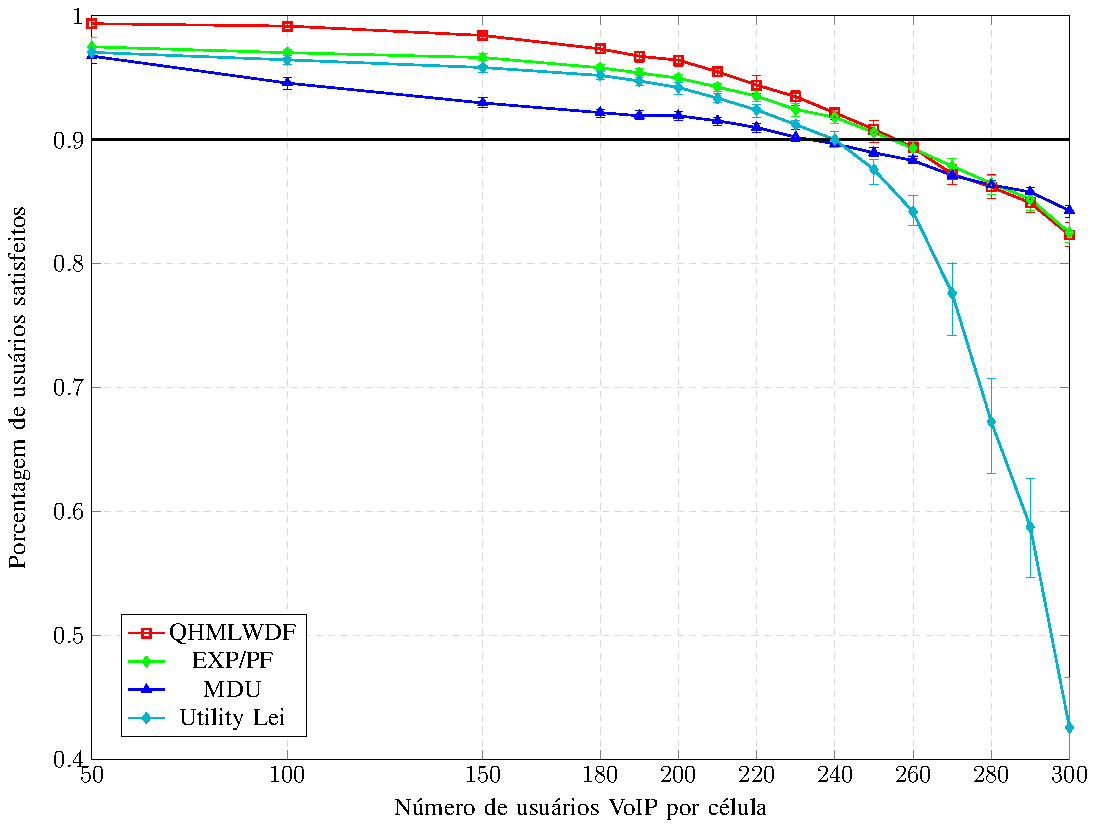
\includegraphics[width=1\textwidth]{figs/VOIPAll.pdf}
	
	{Fonte: Elaborada pelo autor.}
	\label{fig:VoIPAll}
\end{figure}

Os outros três algoritmos estudados conseguem manter a satisfação dos usuários em níveis aceitáveis mesmo após a carga de 240 usuários. Perceba que mesmo com 300 usuários por célula, os algoritmos MDU, EXP/PF e QHMLWDF conseguem uma porcentagem de satisfação acima de 80\%. A última carga com satisfação acima de 90\% para MDU, EXP/PF e QHMLWDF são 240, 260 e 260, respectivamente. O algoritmo EXP/PF consegue atingir esse desempenho devido ao fato de utilizar o atraso do pacote HOL como principal métrica para alocação dos recursos, dando maior prioridade para usuários que estão com atraso maior que a média dos atrasos dos usuários ativos (equação \ref{Eq:EXPPF_RT}), o que faz com que o atraso médio dos usuários seja baixo. O algoritmo MDU alcança esse desempenho utilizando a informação do tamanho da fila dos usuários para fazer a alocação dos recursos (equação \ref{Eq:MDU_RT}), fazendo com que os usuários com maior tamanho da fila tenha maior prioridade e, portanto, mantendo o atraso dos usuários o mais baixo possível. Já o algoritmo QHMLWDF, combina as métricas de atraso do pacote HOL e tamanho da fila de pacotes (equação \ref{Eq:QHMLWDF_RT_NRT}) para manter a PLR dos usuários em baixos níveis,  alcançando bom desempenho neste cenário. 

A conclusão que podemos tirar deste resultado parcial é que as abordagens que utilizam tempo de espera médio (MDU), atraso do pacote HOL (EXP/PF) e tamanho da fila de pacotes e atraso do pacote HOL (QHMLWDF) foram eficazes na tarefa de satisfazer os usuários RT. Apesar do algoritmo \textit{Utility} Lei também utilizar o atraso do pacote HOL como métrica para alocação dos recursos, este algoritmo não obteve resultados tão bons quanto os outros algoritmos, o que pode ser explicado devido ao formato ou inclinação da função de utilidade que foi proposta.

\subsection{Cenário com serviço único NRT}

Nesta seção, mostraremos os resultados obtidos para o cenário composto apenas por usuários utilizando o serviço CBR, ou seja, apenas usuários de um serviço que assumimos como NRT.

A figura \ref{fig:CBRAll} ilustra o gráfico da satisfação dos usuários obtido neste cenário com usuários CBR. A quantidade de usuários por célula foi incrementada de 1 usuário a partir da quantidade inicial de 10 usuários até a carga de 20 usuários. Após isso, a carga de usuários foi incrementada de 2 em 2. Perceba que a granularidade da quantidade de usuários por célula é bem menor para este tipo de serviço. Note também que o eixo que indica a porcentagem de usuários satisfeitos varia de 0.3 até 1, já que nenhum algoritmos apresentou desempenho pior que 30\% dos usuários satisfeitos. 

Pode ser facilmente percebido que o algoritmo EXP/PF apresentou o melhor desempenho neste cenário. O nível de satisfação obtido por este algoritmo ficou acima do nível de satisfação dos outros algoritmos para todas as cargas consideradas. A carga de 26 usuários é a última em que o EXP/PF consegue manter a satisfação acima de 90\%. O principal motivo para isto é que o algoritmo EXPPF utiliza a vazão de dados dos usuários como principal métrica para fazer a alocação dos recursos para o serviço NRT (equação \ref{Eq:EXPPF_NRT}), a qual é a métrica que define a satisfação para esta classe de serviço. Por outro lado, o algoritmo QHMLWDF foi o que obteve pior desempenho. Para a carga máxima analisada de 28 usuários, este algoritmos atingiu menos de 30\% de satisfação, que foi a mais baixa entre os algoritmos analisados. A última carga com satisfação acima de 90\% para o QHMLWDF foi de 14 usuários. Isso ocorreu pelo fato de que este algoritmo foi proposto para manter a PLR dos usuários em baixos níveis por meio do uso das métricas de atraso e tamanho da fila, mas manter a PLR em baixos níveis não garante que usuários NRT estejam satisfeitos. 

Os outros dois algoritmos, a saber MDU e \textit{Utility} Lei, obtiveram resultados medianos neste cenário. Apesar de a última carga em que a satisfação ficou acima de 90\% para o MDU, que foi de 15 usuários CBR, ter sido bem parecida com a do pior algoritmo, o MDU conseguiu sustentar a satisfação dos usuários em níveis mais altos a medida que a carga de usuários foi aumentando. Para o \textit{Utility} Lei, a última carga com satisfação de acima de 90\% foi de 19 usuários CBR.

Uma conclusão parcial obtida depois da observação dos resultados para o cenário com apenas o serviço NRT foi: a melhor abordagem foi a do EXP/PF, que aloca os recursos para os usuários CBR com base no valor da vazão de dados destes usuários, atacando diretamente a métrica que define a satisfação deste tipo de serviço. A abordagem que utiliza tamanho da fila de pacotes e atraso do pacote HOL do QHMLWDF não se mostrou eficaz para este cenário.

\begin{figure}[htb]
	\centering	
	
	\caption[Satisfação dos usuários para cenário com apenas usuários CBR]{Satisfação dos usuários para cenário com apenas usuários CBR.}
	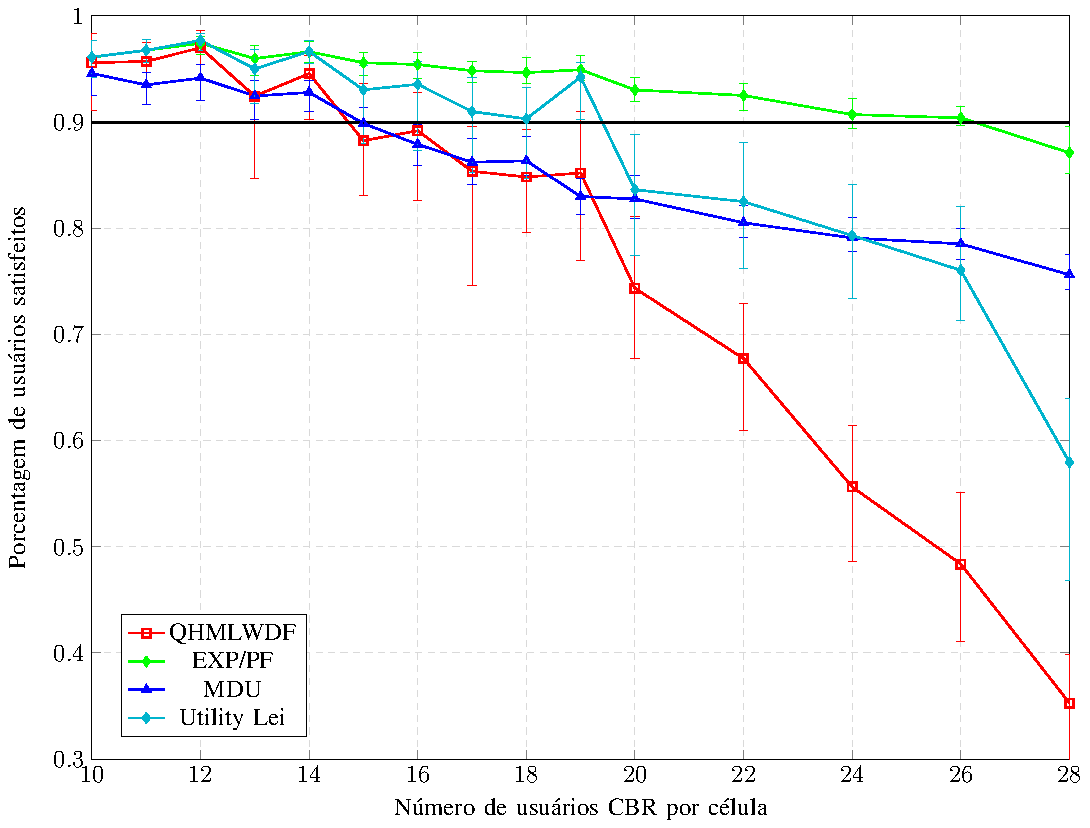
\includegraphics[width=1\textwidth]{figs/CBRAll.pdf}
	
	{Fonte: Elaborada pelo autor.}
	\label{fig:CBRAll}
\end{figure}

\subsection{Cenário com múltiplos serviços}

A partir de agora, iremos mostrar os resultados para cenários compostos por uma mistura de usuários utilizando serviços NRT (CBR) e RT (VoIP). Nos gráficos que ilustram os resultados para este cenário, o eixo das abscissas apresenta a quantidade total de usuários presentes na célula, ou seja, é uma soma da quantidade de usuários CBR e de usuários VoIP. 

A abordagem utilizada para obtenção dos resultados para este cenário foi a seguinte: a quantidade de usuários VoIP era fixada em um determinado número, a saber 100, 150 e 200, e a quantidade de usuários CBR era variada. O critério de parada na variação do número de usuários CBR era o momento em que a satisfação dos dois serviços ficava abaixo de 90\%. Note que o eixo que indica a porcentagem de usuários satisfeitos para este varia de 0 até 1, já que alguns algoritmos apresentaram desempenho bem baixo neste cenário. 

Na figura \ref{fig:100VOIP} mostramos os resultados para o cenário com 100 usuários VoIP e uma quantidade variável de usuários CBR. Pode-se notar que em relação a satisfação do serviço RT, os algoritmos EXP/PF e MDU obtiveram os melhores resultados. Apesar disso, se consideramos a satisfação de uma forma conjunta para os dois serviços, o desempenho do algoritmo EXP/PF foi melhor, o que ocorreu devido ao fato de o EXP/PF utilizar as principais métricas que definem a satisfação de cada tipo serviço, a saber atraso do pacote HOL para o serviço RT e vazão de dados para o serviço NRT. Perceba que os algoritmos EXP/PF e o MDU mantiveram a satisfação do serviço RT sempre acima de 90\%. O MDU consegue manter a satisfação do serviço RT sempre em altos níveis porque este serviço sempre tem maior prioridade na alocação dos recursos (figura \ref{fig:WeightSong}). Já o algoritmo EXP/PF mantém sempre o nível de satisfação do serviço RT mais alto pelo fato de a magnitude da fórmula que define a prioridade do serviço RT (equação \ref{Eq:EXPPF_RT}) ser maior que a magnitude da fórmula para o serviço NRT (equação \ref{Eq:EXPPF_RT}). 

\begin{figure}[hb]
	\centering
	
	\caption[Satisfação dos usuários para cenários com 100 usuários VoIP e um número variável de usuários CBR]{Satisfação dos usuários para cenários com 100 usuários VoIP e um número variável de usuários CBR.}
	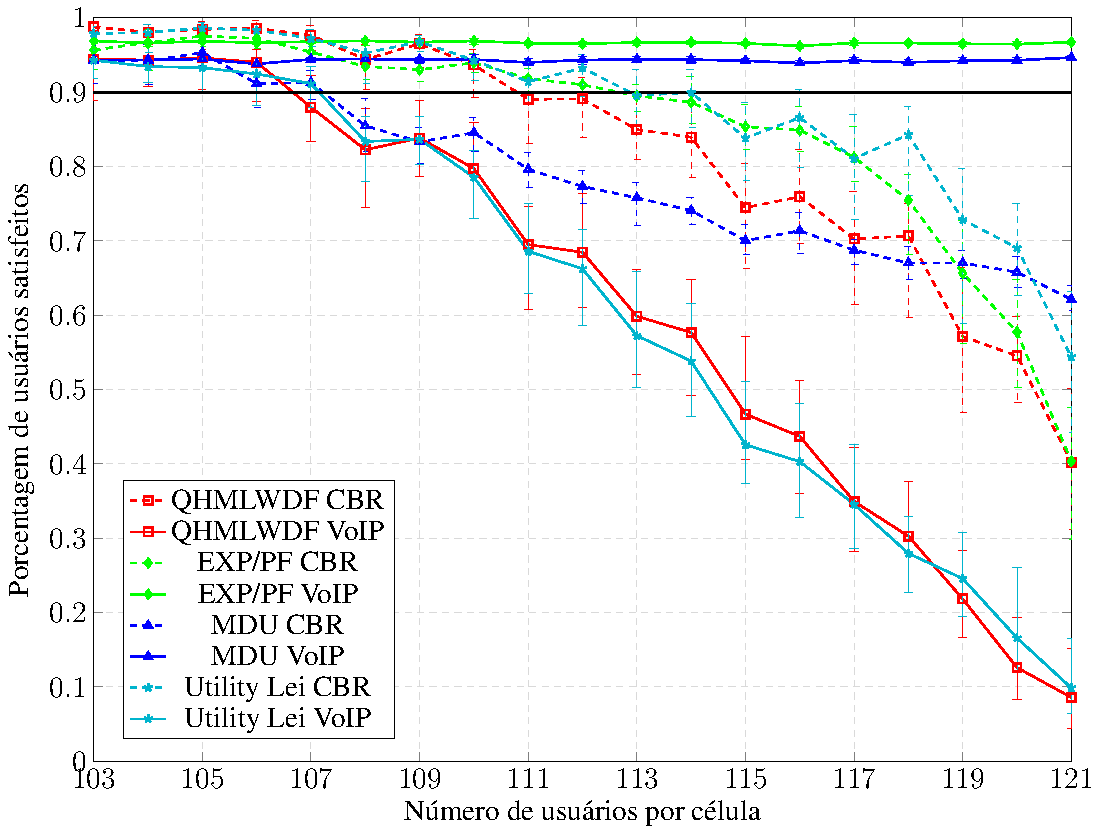
\includegraphics[width=.8\linewidth]{figs/100VOIP.pdf}
	
	{Fonte: Elaborada pelo autor.}
	\label{fig:100VOIP}
\end{figure}

O terceiro melhor desempenho neste cenário foi obtido pelo algoritmo QHMLWDF, enquanto que o algoritmo \textit{Utility} Lei obteve o pior resultado em termos de satisfação conjunta. A última carga de usuários tal que a satisfação ficou acima de 90\% para os dois serviços será mostrada apenas no plano de capacidade conjunta, que será apresentado na próxima subseção. Perceba que para os algoritmos QHMLWDF e \textit{Utility} Lei o nível de satisfação do serviço NRT é sempre mais alto que a satisfação do serviço RT, o que é um comportamento contrário ao apresentado pelos algoritmos EXP/PF e MDU. Para o algoritmo QHMLWDF, isso ocorre pelo fato que este algoritmo utilizar o tamanho da fila para fazer a alocação dos recursos. Como a taxa de geração de pacotes do serviço CBR (512~Kbps, olhar tabela \ref{Tab:Par_CBR}) é maior que a taxa de geração de pacotes do serviço VoIP (16~Kbps, olhar tabela \ref{Tab:Par_VOIP}), o tamanho da fila dos usuários CBR é normalmente maior que a fila dos usuários VOIP, fazendo com que os usuários CBR tenham maior prioridade. Para o algoritmo \textit{Utility} Lei, a satisfação dos usuários NRT é maior que a satisfação dos usuários RT devido ao formato das curvas que definem as prioridades de cada serviço (olhar figura \ref{fig:WeightLEI}). Perceba que quando o atraso do pacote HOL está em valores baixo, o serviço RT tem maior prioridade. Para atrasos mais altos, a prioridade do serviço NRT tende a ser maior. Como o limite de tempo do pacote HOL para o serviço CBR é maior que o limite de tempo do pacote HOL para o serviço VoIP (olhar tabelas \ref{Tab:Par_CBR} e \ref{Tab:Par_VOIP}), a prioridade do serviço CBR tende a ser maior que a prioridade do serviço VOIP. 

\begin{figure}[b]
	\centering
	
	\caption[Satisfação dos usuários para cenários com 150 usuários VoIP e um número variável de usuários CBR]{Satisfação dos usuários para cenários com 150 usuários VoIP e um número variável de usuários CBR.}
	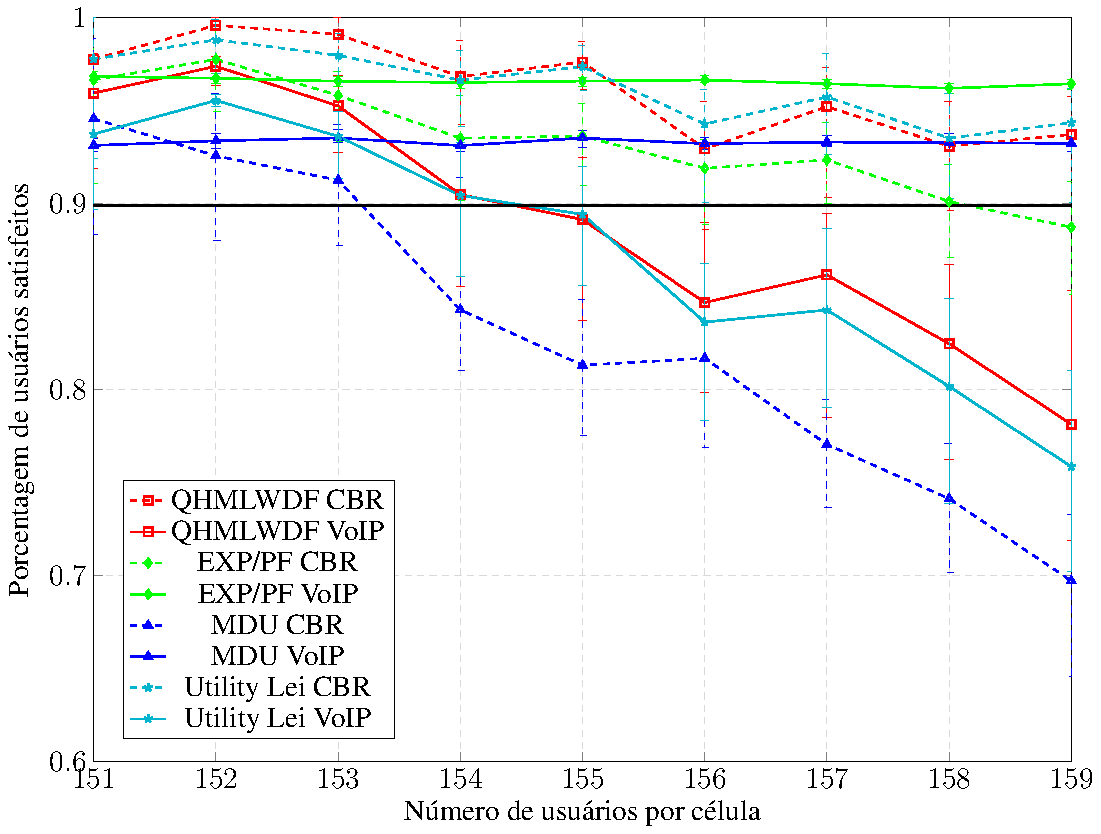
\includegraphics[width=.8\linewidth]{figs/150VOIP.pdf}
	
	{Fonte: Elaborada pelo autor.}	
	\label{fig:150VOIP}
\end{figure}

Na figura \ref{fig:150VOIP} mostramos os resultados para o cenários com 150 usuários VoIP e uma quantidade variável de usuários CBR. Perceba que a medida que vamos aumentando a quantidade fixa de usuários VoIP, a quantidade de usuários CBR suportados vai obviamente diminuindo. Note que o eixo que indica a porcentagem de usuários satisfeitos varia de 0.6 até 1, já que nenhum algoritmos apresentou desempenho pior que 60\% dos usuários satisfeitos. 

Pode-se notar que, em relação a satisfação conjunta, o algoritmo EXP/PF novamente obteve o melhor resultado (o motivo para isso já foi explicado anteriormente). O algoritmo MDU  obteve o pior desempenho para esta quantidade de usuários VoIP. Isso ocorreu porque a prioridade do serviço RT é absolutamente maior que a prioridade do serviço NRT, o que fez com que os usuários CBR não recebessem recursos. Os outros dois algoritmos, QHMLWDF e \textit{Utility} Lei, obtiveram desempenhos similares para este cenários, tanto em relação à satisfação dos usuários CBR quanto em relação à satisfação do serviço RT.

Na figura \ref{fig:200VOIP} mostramos os resultados para o cenários com 200 usuários VoIP e uma quantidade variável de usuários CBR. Para esta quantidade de usuários VoIP, foi necessário apenas que realizássemos simulações com até 5 usuários CBR. Perceba que o eixo que indica a porcentagem de usuários satisfeitos varia de 0.5 até 1.

Note que para este cenário específico, o desempenho de todos os algoritmos, com exceção do algoritmo MDU, foram consideravelmente próximos. O motivo de o desempenho do algoritmo MDU ter sido o pior foi explicado no parágrafo anterior. A última carga suportada com satisfação acima de 90\% obtida pelos algoritmos EXP/PF, QHMLWDF e \textit{Utility} Lei foi de 202 usuários, ou seja, 200 usuários VoIP mais 2 usuários CBR, o que nos leva a concluir que este é o limite máximo de satisfação que pode ser obtido neste cenário, considerando os algoritmos analisados neste estudo. O algoritmo MDU conseguiu apenas manter a satisfação dos usuários VoIP acima de 90\% para este cenário.

Uma forma de condensar os resultados ilustrados nas figuras \ref{fig:VoIPAll}, \ref{fig:CBRAll}, \ref{fig:100VOIP}, \ref{fig:150VOIP}, \ref{fig:200VOIP} em um único gráfico é através do plano de capacidade conjunta, que será definido a partir de agora.

\begin{figure}
	\centering
	
	\caption[Satisfação dos usuários para cenários com 200 usuários VoIP e um número variável de usuários CBR]{Satisfação dos usuários para cenários com 200 usuários VoIP e um número variável de usuários CBR.}
	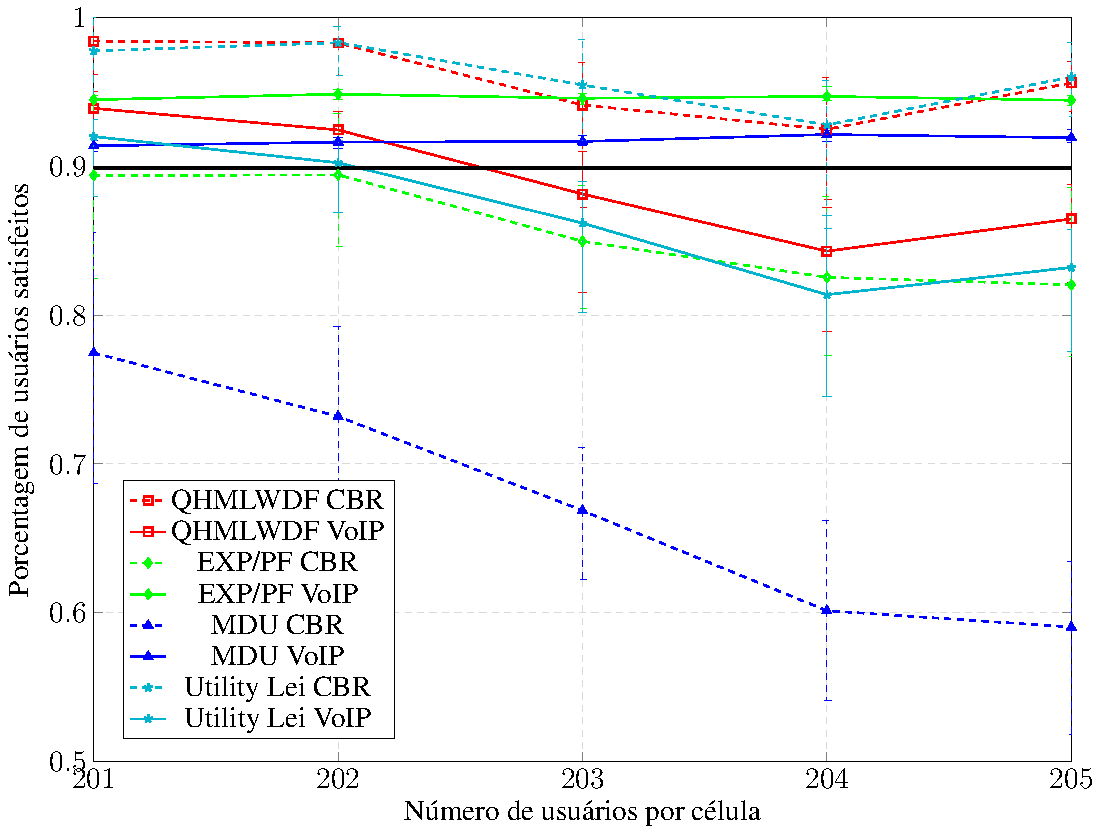
\includegraphics[width=.8\linewidth]{figs/200VOIP.pdf}
	
	{Fonte: Elaborada pelo autor.}
	\label{fig:200VOIP}
\end{figure}

\subsubsection{Plano de capacidade conjunta}

Como já mencionado, o plano de capacidade conjunta é uma ferramenta poderosa para analisar o desempenho de algoritmos de RRA em cenários com múltiplos serviços. Este plano mostra as regiões de capacidade do sistema que podem ser definidas como o número de usuários para o qual os níveis de QoS são mantidos acima de um determinado limiar para todas as classes de serviço ao mesmo tempo.

Considerando os cenários com apenas um tipo de serviço, o ponto de interesse para a construção do plano de capacidade conjunta é aquela carga (número de usuários) tal que os algoritmos são capazes de manter a porcentagem de usuários satisfeitos acima de um determinado nível. 
% Verificar se isto foi dito antes?
Neste trabalho, este nível é 90\% de usuários satisfeitos. Este é o motivo pelo qual uma linha horizontal foi traçada neste nível de satisfação nas figuras \ref{fig:VoIPAll}, \ref{fig:CBRAll}, \ref{fig:100VOIP}, \ref{fig:150VOIP}, \ref{fig:200VOIP}. O valor desta carga dos cenários com um único serviço são utilizadas para achar os pontos que compõem o eixo das abscissas e das ordenadas no plano de capacidade conjunta.

Em relação aos cenários com múltiplos serviços, o valor da capacidade conjunta do sistema é definida como a capacidade máxima que os algoritmos de RRA suportam para ambos os serviços tal que uma determinada qualidade seja garantida para ambos os serviços de forma simultânea. Esta determinada qualidade é definida neste trabalho como nível de QoS e refletida na porcentagem de usuários satisfeitos, que deve estar acima de 90\% para os dois serviços ao mesmo tempo. Os pontos obtidos seguindo este critério são utilizados para construir os pontos do interior do plano de capacidade conjunta.

Na figura \ref{fig:CapPlane} está ilustrado o plano de capacidade conjunta que foi obtido seguindo os critérios definidos nos dois parágrafos anteriores. O desempenho de cada algoritmo de RRA estudado neste trabalho é ilustrado como uma curva de capacidade neste gráfico. Os pontos obtidos a partir das figuras  \ref{fig:VoIPAll} e \ref{fig:CBRAll} foram utilizados para plotar os pontos das ordenadas e abscissas, respectivamente. As cargas que foram extraídas das figuras \ref{fig:100VOIP}, \ref{fig:150VOIP}, \ref{fig:200VOIP} foram utilizados para completar as curvas de capacidade de cada algoritmo de RRA, ligando os pontos extremos das abscissas e coordenadas. Perceba que o intervalo de confiança para este gráfico é representado como intervalos na horizontal em torno de um ponto, representando um variabilidade na quantidade de usuários CBR suportados para uma certa carga de usuários VoIP.

Quanto maior for a área abaixo do gráfico, maior é a porcentagem de usuários satisfeitos respeitando um limite de satisfação mínimo de 90\%. Portanto, pode-se notar que o algoritmo que obteve o melhor desempenho entre todos foi o EXP/PF. Este algoritmo obteve o melhor desempenho para o cenário com serviço único NRT (eixo das abscissas) e também obteve o melhor desempenho para o cenário com serviço único RT (eixo da ordenadas), onde empatou com o algoritmo QHMLWDF. Considerando o cenário com 100 usuários VoIP, o EXP/PF obteve um desempenho 86\% melhor em relação a quantidade de usuários CBR que os algoritmos \textit{Utility} Lei e MDU, que ficaram em segundo lugar neste cenário. Para o cenário com 150 usuários VoIP, o ganho foi de 60\% no número de usuários CBR. Analisando o ganho em relação ao número de usuários VoIP, o máximo obtido foi para uma carga de 13 usuários CBR, onde o ganho foi de 100\% em relação ao número de usuários VoIP. Note também que, de acordo com o intervalo de confiança para os resultados do EXP/PF, existe apenas uma variação de, no máximo, um usuário CBR a mais ou a menos que é suportado para uma determinada carga de usuários VoIP, o que não afetaria a conclusão de que este algoritmo obteve o melhor desempenho.  A razão para o EXP/PF ter obtido o melhor desempenho é que este algoritmo faz a alocação dos recursos para um determinado serviço com base na métrica que define a satisfação para aquele serviço, a saber atraso para o serviço RT e vazão de dados para o serviço NRT. 

\begin{figure}[ht]
	\centering
	
	\caption[Plano de capacidade conjunta]{Plano de capacidade conjunta.}
	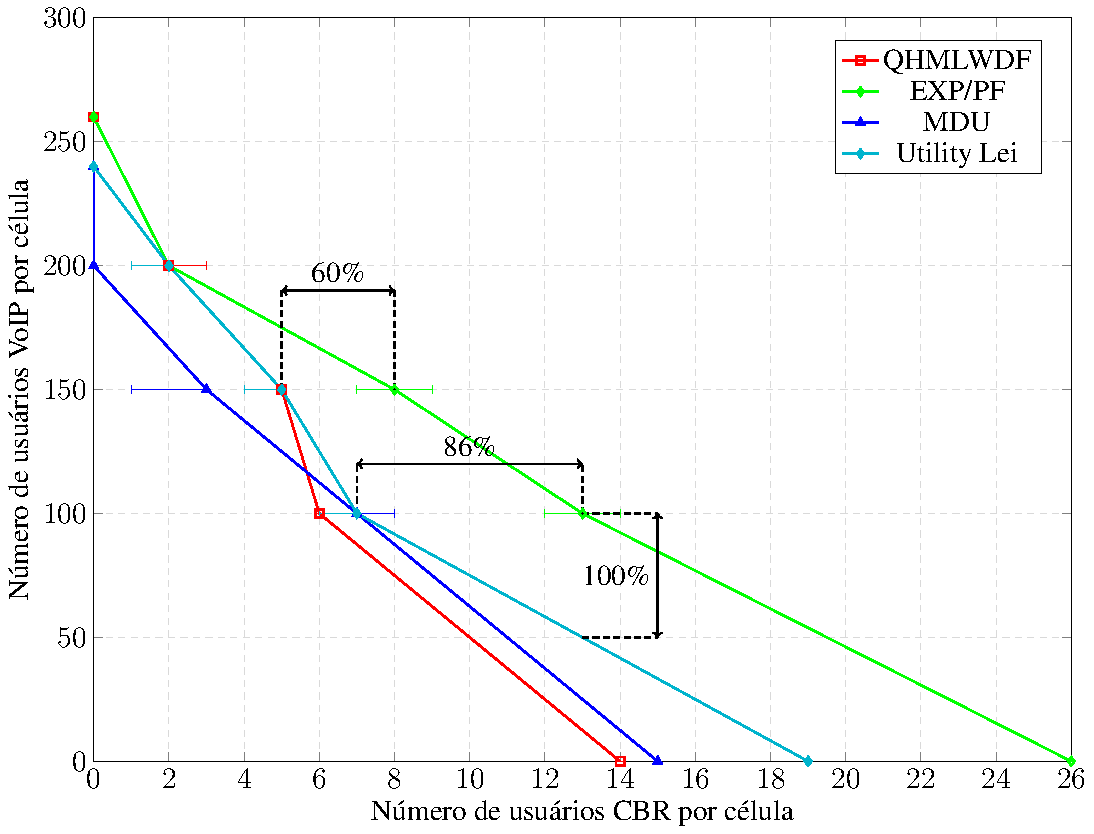
\includegraphics[width=1\linewidth]{figs/CapacityPlane.pdf}
	
	\legend{Fonte: Elaborada pelo autor.}
	\label{fig:CapPlane}
\end{figure}

Em segundo lugar ficou o \textit{Utility} Lei, que obteve o segundo melhor desempenho em todos cenários analisados. Perceba que para este algoritmo, o intervalo de confiança mostra que existe a possibilidade de este algoritmo obter desempenho igual ou pior que o desempenho do QHMLWDF nos cenários analisados, o que poderia alterar a ordem de classificação dos algoritmos segundo seus desempenhos. O principal motivo para este algoritmo não ter conseguido atingir os mesmos resultados que o EXP/PF é que alocação dos recursos para o serviço NRT é também baseada em atraso, assim como para o serviço RT, e não baseada em vazão de dados, como feito no EXP/PF.
 
Nos dois últimos lugares ficaram os algoritmos QHMLWDF e MDU. Estes algoritmos apresentaram os dois piores desempenhos para o cenário com serviço único NRT. Em relação ao cenários com múltiplos serviços, esses algoritmos apresentaram os piores desempenhos. Em relação ao QHMLWDF, isso ocorreu pelo fato de este algoritmo utilizar o tamanho da fila para fazer a alocação de recursos, o que prejudicou bastante o nível de satisfação do serviço RT, já que a taxa de geração de pacotes do serviço CBR é maior que a do serviço VoIP. Em relação ao algoritmo MDU, o principal motivo foi que a prioridade do serviço RT era absolutamente maior que a prioridade do serviço NRT, o que fez com a satisfação do serviço NRT ficasse bastante degradada, como exemplificado na figura \ref{fig:200VOIP}, em que a satisfação do serviço NRT não ficou acima de 90\% para nenhuma carga de usuários CBR. Além disso, note que para o MDU, o intervalo de confiança dos resultados mostra que o desempenho deste algoritmo pode ser ainda significativamente pior no cenário como 150 usuários VoIP, fazendo com que este algoritmo apresente desempenho global ainda pior. 

A conclusão que pode ser obtida a partir deste resultado é que a melhor abordagem que pode ser utilizada para realizar a alocação de recursos em um cenário composto por serviços NRT e RT é a abordagem do EXP/PF, que foi: alocar os recursos para o serviço RT utilizando a métrica de atraso do pacote HOL de cada usuário e alocar os recursos para serviços NRT utilizando a métrica de vazão de dados. Essa abordagem ataca diretamente a métrica de QoS que define a satisfação de cada classe de serviço.